\documentclass[tikz,border=6pt]{standalone}
\usepackage{ctex}
\usepackage{graphicx}
\usepackage{tikz}

\begin{document}
\begin{minipage}{0.98\textwidth}
\centering
\begin{minipage}[t]{0.48\textwidth}
  \centering
  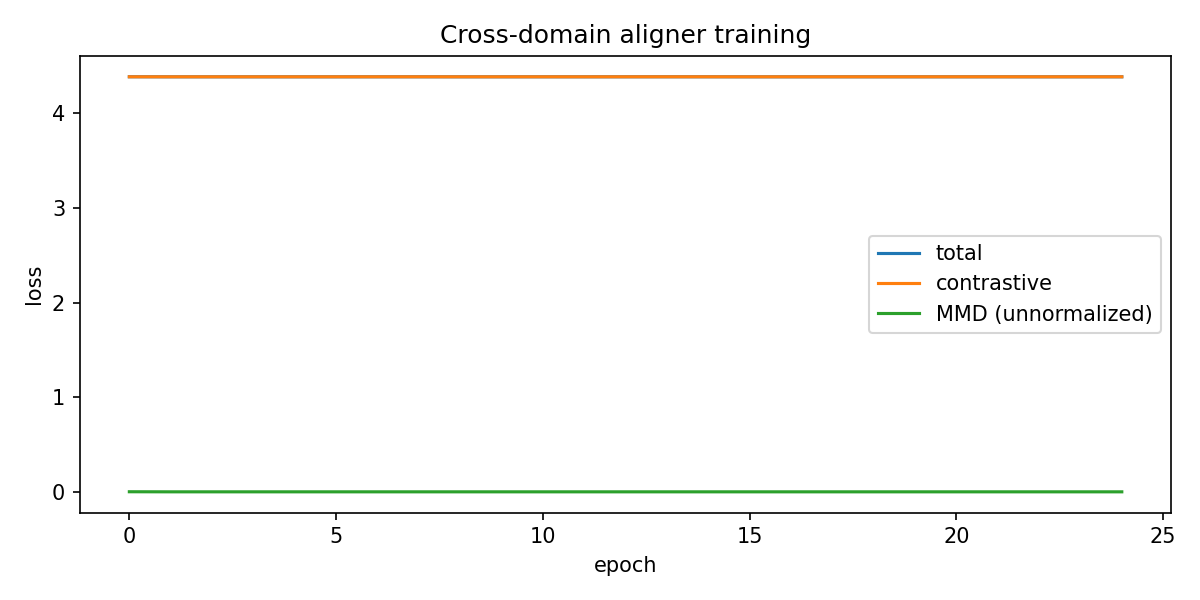
\includegraphics[width=\textwidth]{real-training-images/aligner_loss.png}
  
  \small (a) 对齐器训练损失
\end{minipage}
\hfill
\begin{minipage}[t]{0.48\textwidth}
  \centering
  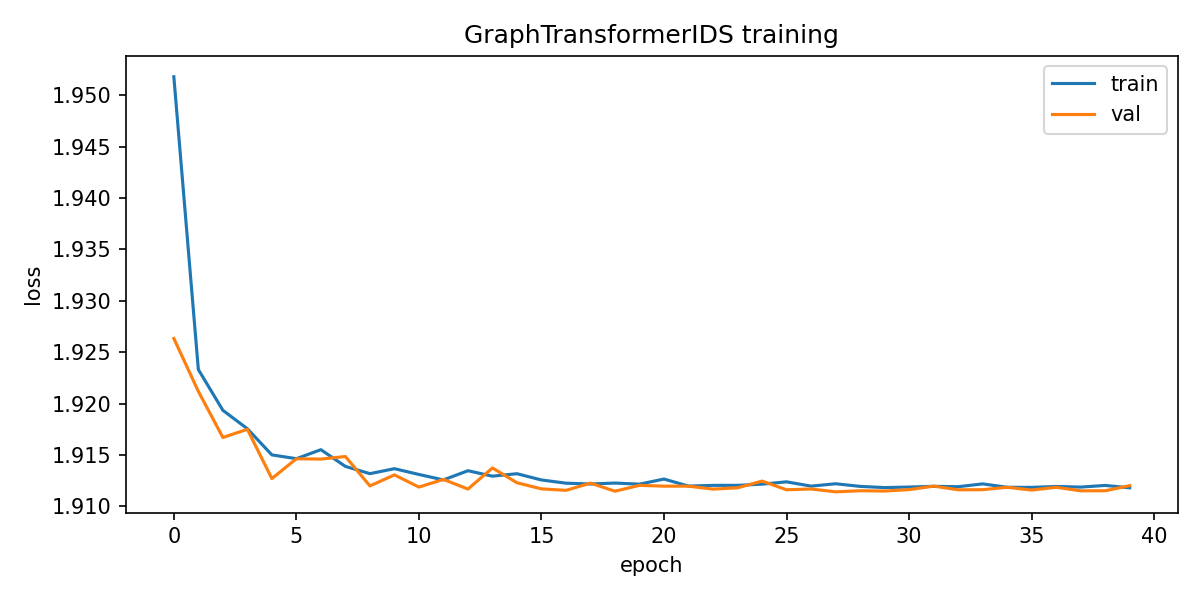
\includegraphics[width=\textwidth]{real-training-images/chain_training.png}
  
  \small (b) 链模型训练过程
\end{minipage}

\vspace{0.7em}

\begin{minipage}[t]{0.48\textwidth}
  \centering
  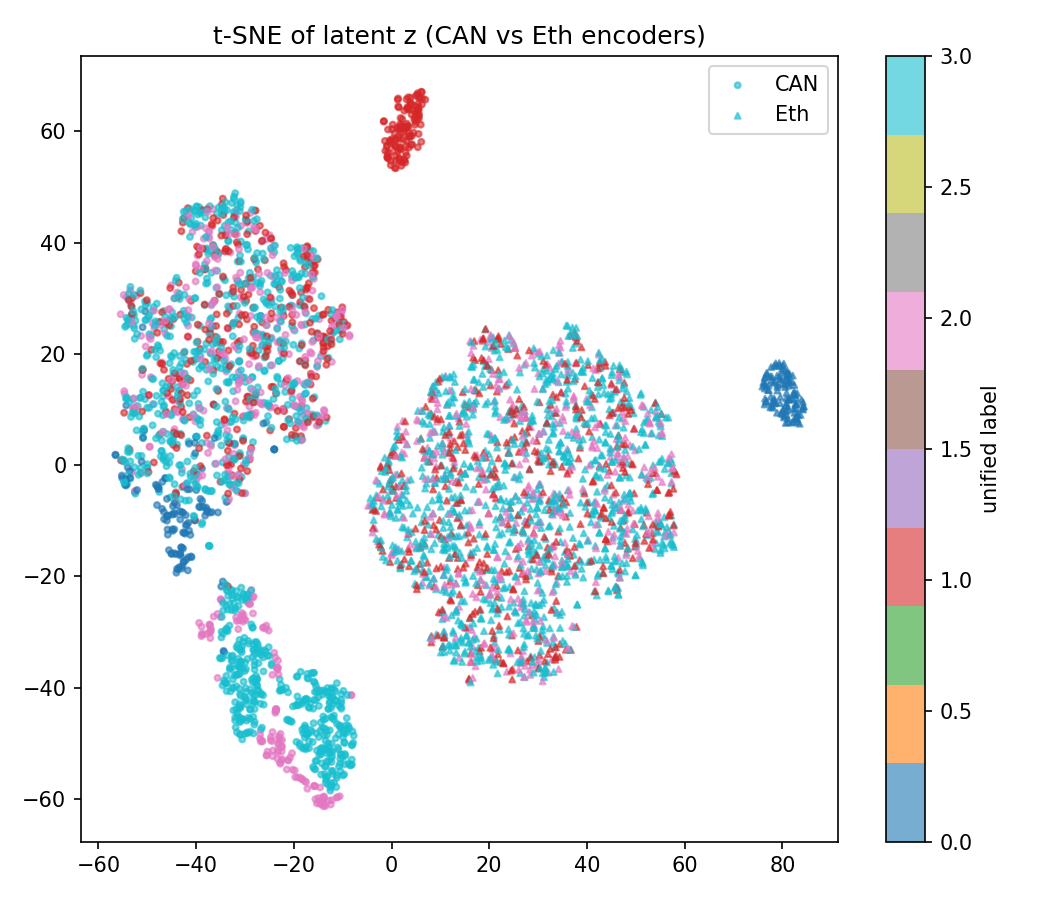
\includegraphics[width=\textwidth]{real-training-images/aligner_latent_tsne.png}
  
  \small (c) 隐空间 t-SNE（跨域对齐）
\end{minipage}
\hfill
\begin{minipage}[t]{0.48\textwidth}
  \centering
  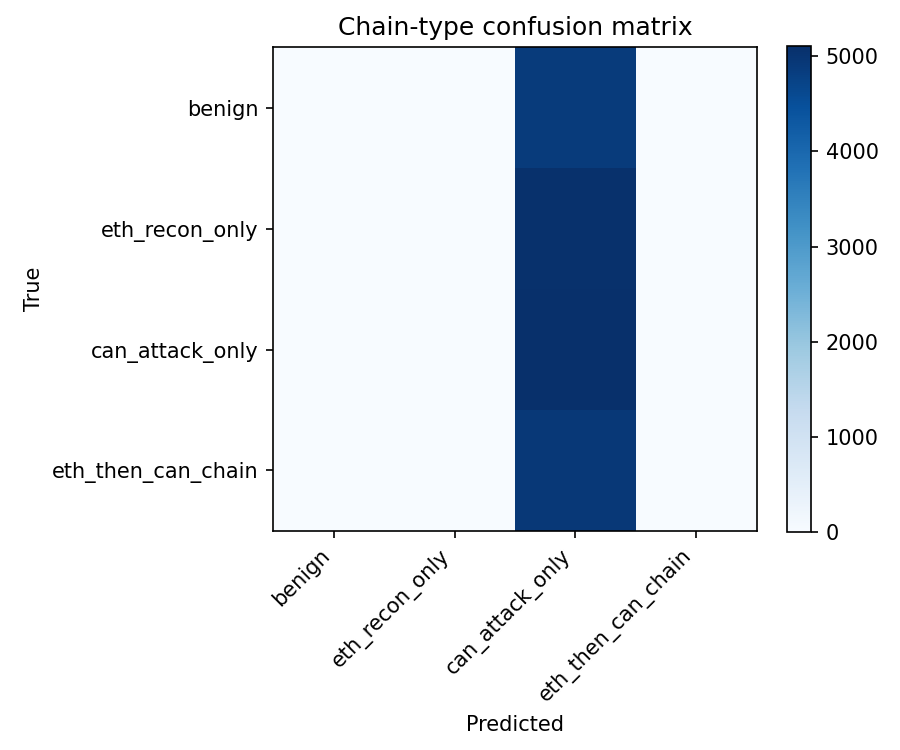
\includegraphics[width=\textwidth]{real-training-images/chain_confusion_matrix.png}
  
  \small (d) 攻击链混淆矩阵
\end{minipage}

\vspace{0.4em}
\begin{tikzpicture}
  \node[draw=black!35, rounded corners=2mm, fill=blue!7, align=left, inner sep=5pt] {
  图中四个面板均来自 \texttt{cross\_domain\_chain/artifacts} 真实训练产物，分别支撑收敛性、对齐性与链分类可分性。};
\end{tikzpicture}
\end{minipage}
\end{document}
